\paragraph{CSE572 Project 3 - Cluster Validation Project}

Mark Khusid

\begin{verbatim}
import pandas as pd
import numpy as np

import matplotlib.pyplot as plt
from matplotlib.pyplot import get_cmap

from scipy.integrate import simpson

from sklearn.impute import KNNImputer
from sklearn.cluster import KMeans, DBSCAN
from sklearn.decomposition import PCA

from sklearn.preprocessing import StandardScaler
\end{verbatim}

\subparagraph{Load the datasets}

\begin{verbatim}
insulin_data = pd.read_csv('InsulinData.csv', low_memory=False)
cgm_data = pd.read_csv('CGMData.csv', low_memory=False)
\end{verbatim}

\subparagraph{View Dataframes}

\begin{verbatim}
insulin_data
\end{verbatim}

\bigskip\noindent
\begin{tabular}{p{\dimexpr 0.045\linewidth-2\tabcolsep}p{\dimexpr 0.045\linewidth-2\tabcolsep}p{\dimexpr 0.045\linewidth-2\tabcolsep}p{\dimexpr 0.045\linewidth-2\tabcolsep}p{\dimexpr 0.045\linewidth-2\tabcolsep}p{\dimexpr 0.045\linewidth-2\tabcolsep}p{\dimexpr 0.045\linewidth-2\tabcolsep}p{\dimexpr 0.045\linewidth-2\tabcolsep}p{\dimexpr 0.045\linewidth-2\tabcolsep}p{\dimexpr 0.045\linewidth-2\tabcolsep}p{\dimexpr 0.045\linewidth-2\tabcolsep}p{\dimexpr 0.045\linewidth-2\tabcolsep}p{\dimexpr 0.045\linewidth-2\tabcolsep}p{\dimexpr 0.045\linewidth-2\tabcolsep}p{\dimexpr 0.045\linewidth-2\tabcolsep}p{\dimexpr 0.045\linewidth-2\tabcolsep}p{\dimexpr 0.045\linewidth-2\tabcolsep}p{\dimexpr 0.045\linewidth-2\tabcolsep}p{\dimexpr 0.045\linewidth-2\tabcolsep}p{\dimexpr 0.045\linewidth-2\tabcolsep}p{\dimexpr 0.045\linewidth-2\tabcolsep}p{\dimexpr 0.045\linewidth-2\tabcolsep}}
\toprule
 & Index & Date & Time & New Device Time & BG Reading (mg/dL) & Linked BG Meter ID & Basal Rate (U/h) & Temp Basal Amount & Temp Basal Type & Temp Basal Duration (h:mm:ss) & ... & Scroll Step Size & Insulin Action Curve Time & Sensor Calibration Rejected Reason & Preset Bolus & Bolus Source & Network Device Associated Reason & Network Device Disassociated Reason & Network Device Disconnected Reason & Sensor Exception & Preset Temp Basal Name \\
\hline
0 & 0 & 2/12/2018 & 13:20:53 & NaN & NaN & NaN & NaN & NaN & NaN & NaN & ... & NaN & NaN & NaN & NaN & NaN & TEMPORARY & NaN & NaN & NaN & NaN \\
\hline
1 & 1 & 2/12/2018 & 13:20:48 & NaN & NaN & NaN & NaN & NaN & NaN & NaN & ... & NaN & NaN & NaN & NaN & NaN & NaN & NaN & NaN & NaN & NaN \\
\hline
2 & 2 & 2/12/2018 & 13:18:48 & NaN & NaN & NaN & 0.0 & NaN & NaN & NaN & ... & NaN & NaN & NaN & NaN & NaN & NaN & NaN & NaN & NaN & NaN \\
\hline
3 & 3 & 2/12/2018 & 13:18:48 & NaN & NaN & NaN & NaN & NaN & NaN & NaN & ... & NaN & NaN & NaN & NaN & NaN & NaN & NaN & NaN & NaN & NaN \\
\hline
4 & 4 & 2/12/2018 & 13:12:33 & NaN & NaN & NaN & NaN & NaN & NaN & NaN & ... & NaN & NaN & NaN & NaN & CLOSED\_LOOP\_MICRO\_BOLUS & NaN & NaN & NaN & NaN & NaN \\
\hline
... & ... & ... & ... & ... & ... & ... & ... & ... & ... & ... & ... & ... & ... & ... & ... & ... & ... & ... & ... & ... & ... \\
\hline
41430 & 22135 & 7/24/2017 & 19:00:01 & NaN & NaN & NaN & 0.0 & NaN & NaN & NaN & ... & NaN & NaN & NaN & NaN & NaN & NaN & NaN & NaN & NaN & NaN \\
\hline
41431 & 22136 & 7/24/2017 & 18:59:44 & NaN & NaN & NaN & 0.0 & NaN & NaN & NaN & ... & NaN & NaN & NaN & NaN & NaN & NaN & NaN & NaN & NaN & NaN \\
\hline
41432 & 22137 & 7/24/2017 & 18:59:44 & NaN & NaN & NaN & NaN & NaN & NaN & NaN & ... & NaN & NaN & NaN & NaN & NaN & NaN & NaN & NaN & NaN & NaN \\
\hline
41433 & 22138 & 7/24/2017 & 18:59:44 & NaN & NaN & NaN & NaN & NaN & NaN & NaN & ... & NaN & NaN & NaN & NaN & NaN & NaN & NaN & NaN & NaN & NaN \\
\hline
41434 & 22139 & 7/24/2017 & 18:59:42 & 7/24/2017 18:59 & NaN & NaN & NaN & NaN & NaN & NaN & ... & NaN & NaN & NaN & NaN & NaN & NaN & NaN & NaN & NaN & NaN \\
\hline
\bottomrule
\end{tabular}

\bigskip

41435 rows $\times$ 47 columns

\begin{verbatim}
#insulin_data['BWZ Carb Input (grams)']
\end{verbatim}

\begin{verbatim}
cgm_data
\end{verbatim}

\bigskip\noindent
\begin{tabular}{p{\dimexpr 0.045\linewidth-2\tabcolsep}p{\dimexpr 0.045\linewidth-2\tabcolsep}p{\dimexpr 0.045\linewidth-2\tabcolsep}p{\dimexpr 0.045\linewidth-2\tabcolsep}p{\dimexpr 0.045\linewidth-2\tabcolsep}p{\dimexpr 0.045\linewidth-2\tabcolsep}p{\dimexpr 0.045\linewidth-2\tabcolsep}p{\dimexpr 0.045\linewidth-2\tabcolsep}p{\dimexpr 0.045\linewidth-2\tabcolsep}p{\dimexpr 0.045\linewidth-2\tabcolsep}p{\dimexpr 0.045\linewidth-2\tabcolsep}p{\dimexpr 0.045\linewidth-2\tabcolsep}p{\dimexpr 0.045\linewidth-2\tabcolsep}p{\dimexpr 0.045\linewidth-2\tabcolsep}p{\dimexpr 0.045\linewidth-2\tabcolsep}p{\dimexpr 0.045\linewidth-2\tabcolsep}p{\dimexpr 0.045\linewidth-2\tabcolsep}p{\dimexpr 0.045\linewidth-2\tabcolsep}p{\dimexpr 0.045\linewidth-2\tabcolsep}p{\dimexpr 0.045\linewidth-2\tabcolsep}p{\dimexpr 0.045\linewidth-2\tabcolsep}p{\dimexpr 0.045\linewidth-2\tabcolsep}}
\toprule
 & Index & Date & Time & New Device Time & BG Reading (mg/dL) & Linked BG Meter ID & Basal Rate (U/h) & Temp Basal Amount & Temp Basal Type & Temp Basal Duration (h:mm:ss) & ... & Scroll Step Size & Insulin Action Curve Time & Sensor Calibration Rejected Reason & Preset Bolus & Bolus Source & Network Device Associated Reason & Network Device Disassociated Reason & Network Device Disconnected Reason & Sensor Exception & Preset Temp Basal Name \\
\hline
0 & 20355 & 2/12/2018 & 13:22:27 & NaN & NaN & NaN & NaN & NaN & NaN & NaN & ... & NaN & NaN & NaN & NaN & NaN & NaN & NaN & NaN & NaN & NaN \\
\hline
1 & 20356 & 2/12/2018 & 13:17:27 & NaN & NaN & NaN & NaN & NaN & NaN & NaN & ... & NaN & NaN & NaN & NaN & NaN & NaN & NaN & NaN & NaN & NaN \\
\hline
2 & 20357 & 2/12/2018 & 13:12:27 & NaN & NaN & NaN & NaN & NaN & NaN & NaN & ... & NaN & NaN & NaN & NaN & NaN & NaN & NaN & NaN & SENSOR\_ERROR & NaN \\
\hline
3 & 20358 & 2/12/2018 & 13:07:27 & NaN & NaN & NaN & NaN & NaN & NaN & NaN & ... & NaN & NaN & NaN & NaN & NaN & NaN & NaN & NaN & SENSOR\_ERROR & NaN \\
\hline
4 & 20359 & 2/12/2018 & 13:02:27 & NaN & NaN & NaN & NaN & NaN & NaN & NaN & ... & NaN & NaN & NaN & NaN & NaN & NaN & NaN & NaN & SENSOR\_ERROR & NaN \\
\hline
... & ... & ... & ... & ... & ... & ... & ... & ... & ... & ... & ... & ... & ... & ... & ... & ... & ... & ... & ... & ... & ... \\
\hline
55338 & 52855 & 7/25/2017 & 12:28:54 & NaN & NaN & NaN & NaN & NaN & NaN & NaN & ... & NaN & NaN & NaN & NaN & NaN & NaN & NaN & NaN & NaN & NaN \\
\hline
55339 & 52856 & 7/25/2017 & 12:23:54 & NaN & NaN & NaN & NaN & NaN & NaN & NaN & ... & NaN & NaN & NaN & NaN & NaN & NaN & NaN & NaN & NaN & NaN \\
\hline
55340 & 52857 & 7/25/2017 & 12:18:54 & NaN & NaN & NaN & NaN & NaN & NaN & NaN & ... & NaN & NaN & NaN & NaN & NaN & NaN & NaN & NaN & NaN & NaN \\
\hline
55341 & 52858 & 7/25/2017 & 12:13:54 & NaN & NaN & NaN & NaN & NaN & NaN & NaN & ... & NaN & NaN & NaN & NaN & NaN & NaN & NaN & NaN & NaN & NaN \\
\hline
55342 & 52859 & 7/25/2017 & 12:08:54 & NaN & NaN & NaN & NaN & NaN & NaN & NaN & ... & NaN & NaN & NaN & NaN & NaN & NaN & NaN & NaN & NaN & NaN \\
\hline
\bottomrule
\end{tabular}

\bigskip

55343 rows $\times$ 47 columns

\subparagraph{EDA on dataframes}

\begin{verbatim}
#insulin_data.info()
\end{verbatim}

\begin{verbatim}
cgm_data.info()
\end{verbatim}

\begin{verbatim}
<class 'pandas.core.frame.DataFrame'>
RangeIndex: 55343 entries, 0 to 55342
Data columns (total 47 columns):
 #   Column                               Non -Null Count  Dtype  
 - - -  - - - - - -                               - - - - - - - - - - - - - -  - - - - -  
 0   Index                                55343 non -null  int64  
 1   Date                                 55343 non -null  object 
 2   Time                                 55343 non -null  object 
 3   New Device Time                      0 non -null      float64
 4   BG Reading (mg/dL)                   0 non -null      float64
 5   Linked BG Meter ID                   0 non -null      float64
 6   Basal Rate (U/h)                     0 non -null      float64
 7   Temp Basal Amount                    0 non -null      float64
 8   Temp Basal Type                      0 non -null      float64
 9   Temp Basal Duration (h:mm:ss)        0 non -null      float64
 10  Bolus Type                           0 non -null      float64
 11  Bolus Volume Selected (U)            0 non -null      float64
 12  Bolus Volume Delivered (U)           0 non -null      float64
 13  Bolus Duration (h:mm:ss)             0 non -null      float64
 14  Prime Type                           0 non -null      float64
 15  Prime Volume Delivered (U)           0 non -null      float64
 16  Alarm                                0 non -null      float64
 17  Suspend                              0 non -null      float64
 18  Rewind                               0 non -null      float64
 19  BWZ Estimate (U)                     0 non -null      float64
 20  BWZ Target High BG (mg/dL)           0 non -null      float64
 21  BWZ Target Low BG (mg/dL)            0 non -null      float64
 22  BWZ Carb Ratio (g/U)                 0 non -null      float64
 23  BWZ Insulin Sensitivity (mg/dL/U)    0 non -null      float64
 24  BWZ Carb Input (grams)               0 non -null      float64
 25  BWZ BG Input (mg/dL)                 0 non -null      float64
 26  BWZ Correction Estimate (U)          0 non -null      float64
 27  BWZ Food Estimate (U)                0 non -null      float64
 28  BWZ Active Insulin (U)               0 non -null      float64
 29  Sensor Calibration BG (mg/dL)        0 non -null      float64
 30  Sensor Glucose (mg/dL)               51175 non -null  float64
 31  ISIG Value                           51175 non -null  float64
 32  Event Marker                         1 non -null      object 
 33  Bolus Number                         0 non -null      float64
 34  Bolus Cancellation Reason            0 non -null      float64
 35  BWZ Unabsorbed Insulin Total (U)     0 non -null      float64
 36  Final Bolus Estimate                 0 non -null      float64
 37  Scroll Step Size                     0 non -null      float64
 38  Insulin Action Curve Time            0 non -null      float64
 39  Sensor Calibration Rejected Reason   0 non -null      float64
 40  Preset Bolus                         0 non -null      float64
 41  Bolus Source                         0 non -null      float64
 42  Network Device Associated Reason     0 non -null      float64
 43  Network Device Disassociated Reason  0 non -null      float64
 44  Network Device Disconnected Reason   0 non -null      float64
 45  Sensor Exception                     4167 non -null   object 
 46  Preset Temp Basal Name               0 non -null      float64
dtypes: float64(42), int64(1), object(4)
memory usage: 19.8+ MB
\end{verbatim}

\subparagraph{Convert `Date' and `Time' columns to datetime format in both datasets for easier manipulation}

\begin{verbatim}
def preprocess_date(date_string):
    date_string = date_string.strip()
    if len(date_string.split()) == 1:
        return date_string
    elif len(date_string.split()) == 2:
        return date_string.split()[0]
\end{verbatim}

\begin{verbatim}
insulin_data['Date'] = insulin_data['Date'].apply(preprocess_date)
\end{verbatim}

\begin{verbatim}
insulin_data['datetime'] = pd.to_datetime(insulin_data['Date'] + ' ' + insulin_data['Time'])

cgm_data['datetime'] = pd.to_datetime(cgm_data['Date'] + ' ' + cgm_data['Time'])
\end{verbatim}

\begin{verbatim}
insulin_data[['Date', 'Time', 'datetime']]
\end{verbatim}

\bigskip\noindent
\begin{tabular}{p{\dimexpr 0.250\linewidth-2\tabcolsep}p{\dimexpr 0.250\linewidth-2\tabcolsep}p{\dimexpr 0.250\linewidth-2\tabcolsep}p{\dimexpr 0.250\linewidth-2\tabcolsep}}
\toprule
 & Date & Time & datetime \\
\hline
0 & 2/12/2018 & 13:20:53 & 2018-02-12 13:20:53 \\
\hline
1 & 2/12/2018 & 13:20:48 & 2018-02-12 13:20:48 \\
\hline
2 & 2/12/2018 & 13:18:48 & 2018-02-12 13:18:48 \\
\hline
3 & 2/12/2018 & 13:18:48 & 2018-02-12 13:18:48 \\
\hline
4 & 2/12/2018 & 13:12:33 & 2018-02-12 13:12:33 \\
\hline
... & ... & ... & ... \\
\hline
41430 & 7/24/2017 & 19:00:01 & 2017-07-24 19:00:01 \\
\hline
41431 & 7/24/2017 & 18:59:44 & 2017-07-24 18:59:44 \\
\hline
41432 & 7/24/2017 & 18:59:44 & 2017-07-24 18:59:44 \\
\hline
41433 & 7/24/2017 & 18:59:44 & 2017-07-24 18:59:44 \\
\hline
41434 & 7/24/2017 & 18:59:42 & 2017-07-24 18:59:42 \\
\hline
\bottomrule
\end{tabular}

\bigskip

41435 rows $\times$ 3 columns

\begin{verbatim}
cgm_data[['Date', 'Time', 'datetime']]
\end{verbatim}

\bigskip\noindent
\begin{tabular}{p{\dimexpr 0.250\linewidth-2\tabcolsep}p{\dimexpr 0.250\linewidth-2\tabcolsep}p{\dimexpr 0.250\linewidth-2\tabcolsep}p{\dimexpr 0.250\linewidth-2\tabcolsep}}
\toprule
 & Date & Time & datetime \\
\hline
0 & 2/12/2018 & 13:22:27 & 2018-02-12 13:22:27 \\
\hline
1 & 2/12/2018 & 13:17:27 & 2018-02-12 13:17:27 \\
\hline
2 & 2/12/2018 & 13:12:27 & 2018-02-12 13:12:27 \\
\hline
3 & 2/12/2018 & 13:07:27 & 2018-02-12 13:07:27 \\
\hline
4 & 2/12/2018 & 13:02:27 & 2018-02-12 13:02:27 \\
\hline
... & ... & ... & ... \\
\hline
55338 & 7/25/2017 & 12:28:54 & 2017-07-25 12:28:54 \\
\hline
55339 & 7/25/2017 & 12:23:54 & 2017-07-25 12:23:54 \\
\hline
55340 & 7/25/2017 & 12:18:54 & 2017-07-25 12:18:54 \\
\hline
55341 & 7/25/2017 & 12:13:54 & 2017-07-25 12:13:54 \\
\hline
55342 & 7/25/2017 & 12:08:54 & 2017-07-25 12:08:54 \\
\hline
\bottomrule
\end{tabular}

\bigskip

55343 rows $\times$ 3 columns

\subparagraph{Search for non-zero BMZ Carb Input Data}

\begin{verbatim}
# This datetime series contains the start of all non NaN and  positive carb input
# data from the column BWZ Carb Input (grams)
meal_times = \
    insulin_data[~insulin_data['BWZ Carb Input (grams)'].isna() & \
    (insulin_data['BWZ Carb Input (grams)'] > 0)]['datetime']
meal_times
\end{verbatim}

\begin{verbatim}
48      2018 -02 -12 09:15:45
129     2018 -02 -12 02:30:55
188     2018 -02 -11 20:33:18
207     2018 -02 -11 18:14:37
222     2018 -02 -11 16:27:04
                ...        
41265   2017 -07 -26 11:24:52
41274   2017 -07 -26 09:27:16
41347   2017 -07 -25 18:31:40
41393   2017 -07 -25 10:39:46
41401   2017 -07 -25 10:21:19
Name: datetime, Length: 747, dtype: datetime64[ns]
\end{verbatim}

\begin{verbatim}
meal_times.index
\end{verbatim}

\begin{verbatim}
Index([   48,   129,   188,   207,   222,   235,   261,   300,   432,   486,
       ...
       41139, 41164, 41172, 41214, 41261, 41265, 41274, 41347, 41393, 41401],
      dtype='int64', length=747)
\end{verbatim}

\subparagraph{Extract Meal Carb Data}

\subparagraph{Obtain Carb Data At Meal Times}

\begin{verbatim}
meal_carb_data = []

for i in meal_times.index:
    meal_carb_data.append(insulin_data['BWZ Carb Input (grams)'].iloc[i])
\end{verbatim}

\begin{verbatim}
len(meal_carb_data)
\end{verbatim}

\begin{verbatim}
747
\end{verbatim}

\begin{verbatim}
meal_carb_data[0:10]
\end{verbatim}

\begin{verbatim}
[np.float64(34.0),
 np.float64(15.0),
 np.float64(71.0),
 np.float64(8.0),
 np.float64(40.0),
 np.float64(9.0),
 np.float64(27.0),
 np.float64(10.0),
 np.float64(40.0),
 np.float64(90.0)]
\end{verbatim}

\begin{verbatim}
len(meal_carb_data)
\end{verbatim}

\begin{verbatim}
747
\end{verbatim}

\subparagraph{Bin Calculations}

\subparagraph{Obtain Max and Min Meal Carbs}

\begin{verbatim}
max_meal_carbs = np.max(meal_carb_data)
max_meal_carbs
\end{verbatim}

\begin{verbatim}
np.float64(129.0)
\end{verbatim}

\begin{verbatim}
min_meal_carbs = np.min(meal_carb_data)
min_meal_carbs
\end{verbatim}

\begin{verbatim}
np.float64(3.0)
\end{verbatim}

\subparagraph{Calculate Number of Bins}

\begin{verbatim}
bin_size = 20 # grams

number_of_bins = int(np.round(((max_meal_carbs - min_meal_carbs) / bin_size), decimals = 0))
number_of_bins
\end{verbatim}

\begin{verbatim}
6
\end{verbatim}

\subparagraph{Create Bins}

\begin{verbatim}
# Create 6 bins in the range of the data
bin_boundaries = np.linspace(min_meal_carbs, max_meal_carbs, 6) 
print("Bin boundaries:", bin_boundaries)
\end{verbatim}

\begin{verbatim}
Bin boundaries: [  3.   28.2  53.4  78.6 103.8 129. ]
\end{verbatim}

\subparagraph{Extract Meal Glucose Data}

\subparagraph{Obtain CGM Data based on Length of After-Meal Window}

\begin{verbatim}
# Initialize meal data list
meal_glucose_data = []
meal_carb_for_analysis_data = []

# Loop through each meal start time
for index, meal_time in meal_times.items():
    # A meal windows is 2 hours long
    meal_window = insulin_data[(insulin_data['datetime'] > meal_time) & 
                               (insulin_data['datetime'] <= (meal_time + pd.Timedelta(hours=2)))]
    #print(meal_window)

    # If that meal window is empty, get corresponding CGM_
    # data that starts at tm -30 and ends at tm+2hrs
    if meal_window.empty:
        # Step 4 condition (a): No meal between tm and tm+2hrs, use this stretch as meal data
        meal_cgm_data = cgm_data[(cgm_data['datetime'] >= (meal_time - pd.Timedelta(minutes=30))) & 
                                 (cgm_data['datetime'] <= (meal_time + pd.Timedelta(hours=2)))]
    else:
        # Step 4 check for condition (b) or (c)
        next_meal_time = meal_window.iloc[0]['datetime']
        if next_meal_time < (meal_time + pd.Timedelta(hours=2)):
            # condition (b): There is a meal at tp between tm and tm+2hrs, use tp data
            meal_time = next_meal_time
            meal_cgm_data = cgm_data[(cgm_data['datetime'] >= (meal_time - pd.Timedelta(minutes=30))) & 
                                     (cgm_data['datetime'] <= (meal_time + pd.Timedelta(hours=2)))]
        # Condition (c): There is a meal exactly at tm+2hrs, use tm+1hr 30min to tm+4hrs
        elif next_meal_time == (meal_time + pd.Timedelta(hours=2)):
            meal_cgm_data = cgm_data[(cgm_data['datetime'] >= (meal_time + pd.Timedelta(hours=1, minutes=30))) & 
                                     (cgm_data['datetime'] <= (meal_time + pd.Timedelta(hours=4)))]

    # Check if the extracted data has the correct number of points (30 for meal data)
    if len(meal_cgm_data) == 30:
        #print(f"Meal Time Data {meal_time} has {len(meal_cgm_data)} number of points.")
        meal_glucose_data.append(meal_cgm_data['Sensor Glucose (mg/dL)'].values)
        meal_carb_for_analysis_data.append(insulin_data['BWZ Carb Input (grams)'].iloc[index])
\end{verbatim}

\subparagraph{Get Length of Meal Data CGM Values}

\begin{verbatim}
len(meal_glucose_data)
\end{verbatim}

\begin{verbatim}
715
\end{verbatim}

\begin{verbatim}
len(meal_carb_for_analysis_data)
\end{verbatim}

\begin{verbatim}
715
\end{verbatim}

\subparagraph{Assign Each Meal to a Bin}

\begin{verbatim}
meal_bin_indices = np.digitize(meal_carb_for_analysis_data, bin_boundaries, right=False)
meal_bin_indices = meal_bin_indices - 1
print("Bin indices:", meal_bin_indices)
\end{verbatim}

\begin{verbatim}
Bin indices: [1 0 2 0 1 0 0 1 3 2 0 2 0 1 1 1 0 0 0 2 1 1 0 2 1 1 1 0 1 0 0 0 1 0 2 3 0
 2 0 0 0 0 3 0 2 0 3 0 0 1 0 2 0 0 0 0 0 0 1 0 1 0 0 2 0 1 0 0 0 0 0 1 0 1
 1 1 3 1 0 1 1 1 0 1 2 1 1 0 0 1 0 0 1 1 2 1 1 1 0 3 0 0 1 1 0 0 2 1 1 0 0
 0 1 1 0 1 0 1 0 2 0 1 1 0 1 1 0 0 0 1 1 0 1 0 3 0 1 0 1 0 1 0 1 0 3 0 2 1
 1 0 0 1 0 0 0 0 0 0 1 1 0 0 0 0 3 0 0 3 0 1 0 0 1 2 0 0 2 0 0 1 0 0 1 0 0
 1 2 0 1 0 0 0 0 0 2 0 2 0 0 1 0 1 1 0 0 3 0 0 0 0 0 0 3 3 1 2 0 0 2 0 0 1
 2 0 2 0 0 1 0 2 0 0 0 0 0 2 0 0 1 0 1 0 2 0 3 0 2 1 1 0 0 2 0 2 2 0 0 1 0
 1 1 0 1 0 1 0 0 1 1 2 1 0 1 2 2 0 1 3 1 0 3 0 1 2 0 1 0 1 2 0 0 0 0 0 0 0
 0 3 0 0 2 0 1 2 0 2 0 0 2 2 4 0 2 1 1 0 2 1 2 1 0 0 2 2 1 0 0 0 1 2 0 1 0
 2 2 0 0 1 2 0 0 0 0 2 0 0 0 0 1 1 3 0 3 2 0 0 1 1 0 2 1 2 0 3 0 0 1 2 0 0
 0 1 0 0 0 1 0 0 1 2 1 1 2 0 1 1 0 2 1 0 1 3 1 0 1 2 0 0 1 0 1 0 0 1 0 3 0
 0 0 0 2 0 1 2 3 1 3 2 1 2 0 3 0 0 0 0 2 0 0 3 3 0 0 1 1 0 2 0 2 2 0 1 2 2
 2 0 2 2 2 0 2 2 2 1 0 0 2 0 2 2 2 2 2 2 0 0 1 1 1 0 3 0 2 1 0 2 1 2 2 1 1
 0 1 0 0 1 1 1 0 1 1 0 1 0 2 1 0 0 0 1 2 1 1 1 2 0 1 1 2 3 1 1 2 3 1 1 1 0
 1 0 1 2 2 1 2 2 0 1 0 1 0 3 0 1 1 1 3 1 0 1 2 0 3 0 1 0 0 1 3 1 3 2 1 2 0
 0 0 3 0 2 2 0 1 0 0 1 2 3 2 0 1 3 1 0 1 0 3 4 4 2 1 3 0 0 3 1 1 3 3 1 1 0
 2 0 1 1 2 3 2 1 1 0 3 1 0 1 1 1 0 0 3 1 1 0 5 0 3 1 0 0 1 0 0 0 0 2 1 0 1
 1 0 1 1 0 1 0 0 1 0 2 2 0 2 1 2 1 1 2 0 2 0 1 1 0 2 0 0 0 2 0 2 2 3 2 0 1
 1 1 1 1 2 0 0 0 1 1 2 0 3 1 0 1 1 1 1 1 3 3 2 0 1 0 1 3 1 0 0 4 1 0 3 0 0
 4 2 2 2 2 1 0 2 2 0 2 4]
\end{verbatim}

\begin{verbatim}
len(meal_bin_indices)
\end{verbatim}

\begin{verbatim}
715
\end{verbatim}

\begin{verbatim}
min(meal_bin_indices)
\end{verbatim}

\begin{verbatim}
np.int64(0)
\end{verbatim}

\begin{verbatim}
max(meal_bin_indices)
\end{verbatim}

\begin{verbatim}
np.int64(5)
\end{verbatim}

\subparagraph{Create Meal Data Matrix}

\begin{verbatim}
meal_data_matrix = np.vstack(meal_glucose_data)
meal_data_matrix
\end{verbatim}

\begin{verbatim}
array([[ nan,  nan, 124., ..., 178., 184., 185.],
       [121., 120., 115., ...,  86.,  84.,  80.],
       [287., 288., 289., ..., 201., 189., 162.],
       ...,
       [274., 278., 283., ..., 268., 281., 292.],
       [223., 222., 222., ..., 324., 326., 328.],
       [ 82.,  85.,  92., ..., 164., 163., 155.]])
\end{verbatim}

\begin{verbatim}
meal_data_matrix.shape
\end{verbatim}

\begin{verbatim}
(715, 30)
\end{verbatim}

\subparagraph{Handle Missing Data}

We will use a strategy of deleting rows of data that have more than 10\% of bad data.  If less than 10\%, we will use KNN with a nearest neighbor hyperparameter (K=7).

\subparagraph{Define Threshold for Dumping Data}

\begin{verbatim}
# 10%
dump_thresold = 0.1
\end{verbatim}

\subparagraph{Create KNN Imputer}

\begin{verbatim}
knn_imputer = KNNImputer(n_neighbors=7)
\end{verbatim}

\subparagraph{Parse Meal Data and Handle Missing Values}

\begin{verbatim}
cleaned_meal_glucose_data = []
cleaned_meal_bin_indices = []
cleaned_meal_carb_for_analysis_data = []

for index, row in enumerate(meal_data_matrix):
    
    proportion_missing_data = np.isnan(row).mean()

    if proportion_missing_data > dump_thresold:

        # Ignore this row
        #print(f"Ignoring row with {proportion_missing_data*100:.2f}% missing data")
        continue

    else:
        # The data is good, use it
        cleaned_meal_glucose_data.append(row)
        cleaned_meal_carb_for_analysis_data.append(meal_carb_for_analysis_data[index])
        cleaned_meal_bin_indices.append(meal_bin_indices[index])
\end{verbatim}

\begin{verbatim}
len(cleaned_meal_glucose_data)
\end{verbatim}

\begin{verbatim}
619
\end{verbatim}

\begin{verbatim}
len(cleaned_meal_bin_indices)
\end{verbatim}

\begin{verbatim}
619
\end{verbatim}

\subparagraph{Convert Cleaned Meal Glucose Data List into a Matrix}

\begin{verbatim}
cleaned_meal_glucose_data_matrix = \
    np.array(cleaned_meal_glucose_data)
\end{verbatim}

\begin{verbatim}
cleaned_meal_glucose_data_matrix.shape
\end{verbatim}

\begin{verbatim}
(619, 30)
\end{verbatim}

\subparagraph{Use KNN to Impute NaNs in Cleaned Meal Data}

\begin{verbatim}
cleaned_imputed_meal_glucose_data_matrix = \
    knn_imputer.fit_transform(cleaned_meal_glucose_data_matrix)
\end{verbatim}

\begin{verbatim}
#cleaned_imputed_meal_glucose_data_matrix[0]
\end{verbatim}

\subparagraph{Feature Extraction}

\subparagraph{Define Feature Extractor Helper Functions}

\begin{verbatim}
def compute_first_derivative(glucose_data, delta_t=5):
    return np.diff(glucose_data) / delta_t
\end{verbatim}

\begin{verbatim}
def compute_second_derivative(glucose_values, delta_t=5):
    second_derivative = np.zeros(len(glucose_values) - 2)
    for i in range(1, len(glucose_values) - 1):
        second_derivative[i - 1] = \
            (glucose_values[i + 1] - 2 * glucose_values[i] + glucose_values[i - 1]) / (delta_t ** 2)
    return second_derivative
\end{verbatim}

\begin{verbatim}
def compute_AUC(glucose_values, delta_t=5):
    return simpson(glucose_values, dx=delta_t)
\end{verbatim}

\subparagraph{Define Feature Extractor Function}

\begin{verbatim}
def feature_extractor(data_matrix):

    features = []

    for row in data_matrix:
        mean_glucose = np.mean(row)
        std_glucose  = np.std(row)
        max_glucose  = np.max(row)
        min_glucose  = np.min(row)
        
        first_derivative = compute_first_derivative(row)
        mean_first_derivate = np.mean(first_derivative)

        if len(row) > 2:
            second_derivative = compute_second_derivative(row)
            mean_second_derivative = np.mean(second_derivative)
        else:
            mean_second_derivative = 0

        AUC = compute_AUC(row)

        time_to_peak = np.argmax(row)

        features_vector = [
            mean_glucose,
            std_glucose,
            max_glucose,
            min_glucose,
            mean_first_derivate,
            mean_second_derivative,
            AUC,
            time_to_peak
        ]

        features.append(features_vector)
    
    return np.array(features)
\end{verbatim}

\subparagraph{Get Feature Matrix for Cleaned Imputed Meal Data}

\begin{verbatim}
meal_glucose_features_matrix = \
    feature_extractor(cleaned_imputed_meal_glucose_data_matrix)
#len(meal_gluxose_features_matrix[0])
\end{verbatim}

\begin{verbatim}
len(cleaned_imputed_meal_glucose_data_matrix)
\end{verbatim}

\begin{verbatim}
619
\end{verbatim}

\begin{verbatim}
len(meal_glucose_features_matrix)
\end{verbatim}

\begin{verbatim}
619
\end{verbatim}

\begin{verbatim}
len(cleaned_meal_carb_for_analysis_data)
\end{verbatim}

\begin{verbatim}
619
\end{verbatim}

\begin{verbatim}
len(cleaned_meal_bin_indices)
\end{verbatim}

\begin{verbatim}
619
\end{verbatim}

\begin{verbatim}
cleaned_meal_carb_for_analysis_data[0:5]
\end{verbatim}

\begin{verbatim}
[np.float64(15.0),
 np.float64(71.0),
 np.float64(8.0),
 np.float64(10.0),
 np.float64(40.0)]
\end{verbatim}

\begin{verbatim}
cleaned_meal_bin_indices[0:5]
\end{verbatim}

\begin{verbatim}
[np.int64(0), np.int64(2), np.int64(0), np.int64(0), np.int64(1)]
\end{verbatim}

\subparagraph{Normalize the Feature Matrix}

\begin{verbatim}
scaler = StandardScaler()
scaled_meal_glucose_features_matrix = \
    scaler.fit_transform(meal_glucose_features_matrix)
\end{verbatim}

\begin{verbatim}
meal_glucose_features_matrix[0:5]
\end{verbatim}

\begin{verbatim}
array([[ 8.98190476e+01,  1.91175360e+01,  1.31000000e+02,
         4.90000000e+01, -2.82758621e -01, -4.28571429e -03,
         1.30310714e+04,  9.00000000e+00],
       [ 2.14033333e+02,  4.45903452e+01,  2.89000000e+02,
         1.53000000e+02, -8.62068966e -01, -4.00000000e -02,
         3.10037500e+04,  2.00000000e+00],
       [ 1.46833333e+02,  2.61484013e+01,  1.89000000e+02,
         1.00000000e+02, -2.89655172e -01,  5.28571429e -02,
         2.11329167e+04,  0.00000000e+00],
       [ 2.01700000e+02,  1.21714146e+01,  2.21000000e+02,
         1.77000000e+02,  1.51724138e -01,  1.85714286e -02,
         2.92870833e+04,  1.80000000e+01],
       [ 8.82000000e+01,  3.36426317e+01,  1.69000000e+02,
         5.90000000e+01,  6.13793103e -01, -4.28571429e -03,
         1.26495833e+04,  2.80000000e+01]])
\end{verbatim}

\begin{verbatim}
scaled_meal_glucose_features_matrix[0:5]
\end{verbatim}

\begin{verbatim}
array([[ -1.35358146, -0.64438944, -1.34072717, -1.28537305, -0.95960069,
        -0.264903  , -1.34238262, -0.8852873 ],
       [ 0.90939359,  0.73923035,  1.18551723,  0.73417365, -1.97024273,
        -2.54215225,  0.89878287, -1.54257823],
       [ -0.31487721, -0.26249029, -0.41337163, -0.29501842, -0.97163214,
         3.37869579, -0.33209493, -1.73037564],
       [ 0.68470103, -1.02168552,  0.09827281,  1.20022289, -0.20161916,
         1.19253652,  0.68471716, -0.04019896],
       [ -1.38307778,  0.14457771, -0.7331494 , -1.09118587,  0.60448818,
        -0.264903  , -1.3899536 ,  0.89878808]])
\end{verbatim}

\subparagraph{Cluster the Data}

\subparagraph{Convert Bins List into a Column Matrix}

\begin{verbatim}
meal_bin_indices_column_vector = \
    np.array(cleaned_meal_bin_indices).reshape( -1, 1)
\end{verbatim}

\begin{verbatim}
meal_bin_indices_column_vector[0:5]
\end{verbatim}

\begin{verbatim}
array([[0],
       [2],
       [0],
       [0],
       [1]])
\end{verbatim}

\subparagraph{Add Bin Data to Feature Data}

\begin{verbatim}
#combined_feature_bin_data = \
#    np.hstack((meal_gluxose_features_matrix, meal_bin_indices_column_vector))
combined_feature_bin_data = meal_glucose_features_matrix
#combined_feature_bin_data = scaled_meal_glucose_features_matrix
\end{verbatim}

\begin{verbatim}
combined_feature_bin_data[0:5]
\end{verbatim}

\begin{verbatim}
array([[ 8.98190476e+01,  1.91175360e+01,  1.31000000e+02,
         4.90000000e+01, -2.82758621e -01, -4.28571429e -03,
         1.30310714e+04,  9.00000000e+00],
       [ 2.14033333e+02,  4.45903452e+01,  2.89000000e+02,
         1.53000000e+02, -8.62068966e -01, -4.00000000e -02,
         3.10037500e+04,  2.00000000e+00],
       [ 1.46833333e+02,  2.61484013e+01,  1.89000000e+02,
         1.00000000e+02, -2.89655172e -01,  5.28571429e -02,
         2.11329167e+04,  0.00000000e+00],
       [ 2.01700000e+02,  1.21714146e+01,  2.21000000e+02,
         1.77000000e+02,  1.51724138e -01,  1.85714286e -02,
         2.92870833e+04,  1.80000000e+01],
       [ 8.82000000e+01,  3.36426317e+01,  1.69000000e+02,
         5.90000000e+01,  6.13793103e -01, -4.28571429e -03,
         1.26495833e+04,  2.80000000e+01]])
\end{verbatim}

\subparagraph{K-Means Clustering}

\begin{verbatim}
number_of_bins
\end{verbatim}

\begin{verbatim}
6
\end{verbatim}

\begin{verbatim}
cleaned_meal_bin_indices[0:5]
\end{verbatim}

\begin{verbatim}
[np.int64(0), np.int64(2), np.int64(0), np.int64(0), np.int64(1)]
\end{verbatim}

\begin{verbatim}
max(cleaned_meal_bin_indices)
\end{verbatim}

\begin{verbatim}
np.int64(5)
\end{verbatim}

\begin{verbatim}
min(cleaned_meal_bin_indices)
\end{verbatim}

\begin{verbatim}
np.int64(0)
\end{verbatim}

\begin{verbatim}
# Set the number of clusters for K -means
k = int(number_of_bins)
y_bins = np.array(cleaned_meal_bin_indices)

# Initialize and fit KMeans
kmeans = KMeans(n_clusters=k, random_state=123)
y_kmeans = kmeans.fit_predict(scaled_meal_glucose_features_matrix)
\end{verbatim}

\begin{verbatim}
y_kmeans[0:5]
\end{verbatim}

\begin{verbatim}
array([5, 4, 5, 4, 2], dtype=int32)
\end{verbatim}

\begin{verbatim}
y_kmeans.shape
\end{verbatim}

\begin{verbatim}
(619,)
\end{verbatim}

\begin{verbatim}
# Set the number of clusters for K -means
k = int(number_of_bins)
y_bins = np.array(cleaned_meal_bin_indices)

# Initialize and fit KMeans
kmeans = KMeans(n_clusters=k, random_state=123)
y_kmeans = kmeans.fit_predict(scaled_meal_glucose_features_matrix)

# Get cluster labels and centroids
kmeans_cluster_labels = kmeans.labels_
centroids = kmeans.cluster_centers_

pca = PCA(n_components=2)
X_pca_kmeans = pca.fit_transform(scaled_meal_glucose_features_matrix)

# Plotting the clusters found by k -means
plt.figure(figsize=(10, 5))

# Get the viridis color map and extract six colors from it
viridis = get_cmap('viridis', k)
colors = [viridis(i) for i in range(k)]

# Subplot 1: Scatter plot by k -means clusters
plt.subplot(1, 2, 1)
for i in range(k):
    cluster_points = X_pca_kmeans[y_kmeans == i]
    plt.scatter(cluster_points[:, 0], cluster_points[:, 1], 
                color=colors[i], label=f'Cluster {i + 1}', alpha=0.6, marker='o')

# Plotting the centroids after PCA transformation
centroids_pca = pca.transform(centroids)
plt.scatter(centroids_pca[:, 0], centroids_pca[:, 1], 
            color='red', edgecolor='black', marker='X', s=100, label='Centroids')

plt.title("K -Means Clusters")
plt.xlabel('PCA Component 1')
plt.ylabel('PCA Component 2')
plt.legend()

plt.show()
\end{verbatim}

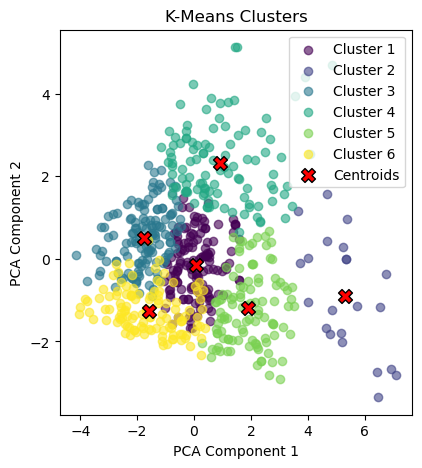
\includegraphics[width=0.7\linewidth]{files/314ad239476762aabac2233ebe6b5061.png}

\begin{verbatim}
# Set the number of clusters for K -means
k = int(number_of_bins)
y_bins = np.array(cleaned_meal_bin_indices)

# Initialize and fit KMeans
kmeans = KMeans(n_clusters=k, random_state=123)
y_kmeans = kmeans.fit_predict(scaled_meal_glucose_features_matrix)

# Get cluster labels and centroids
kmeans_cluster_labels = kmeans.labels_
centroids = kmeans.cluster_centers_

pca = PCA(n_components=2)
X_pca = pca.fit_transform(scaled_meal_glucose_features_matrix)

# Plotting the clusters found by k -means
plt.figure(figsize=(10, 5))

# Subplot 1: Scatter plot by original bins
plt.subplot(1, 2, 1)
plt.scatter(
    np.arange(0, y_bins.shape[0]),
    y_bins,
    c=y_bins,
    cmap='rainbow',
    marker='o')
plt.title("Original Bins")
plt.xlabel("Sample Index")
plt.ylabel("Bin Label")

# Subplot 2: Scatter plot by k -means clusters
plt.subplot(1, 2, 2)
plt.scatter(
    np.arange(0, y_kmeans.shape[0]),
    y_kmeans,
    c=y_kmeans,
    cmap='rainbow',
    marker='o')
plt.title("K -Means Clusters")
plt.xlabel("Sample Index")
plt.ylabel("Bin Label")

plt.show()
\end{verbatim}

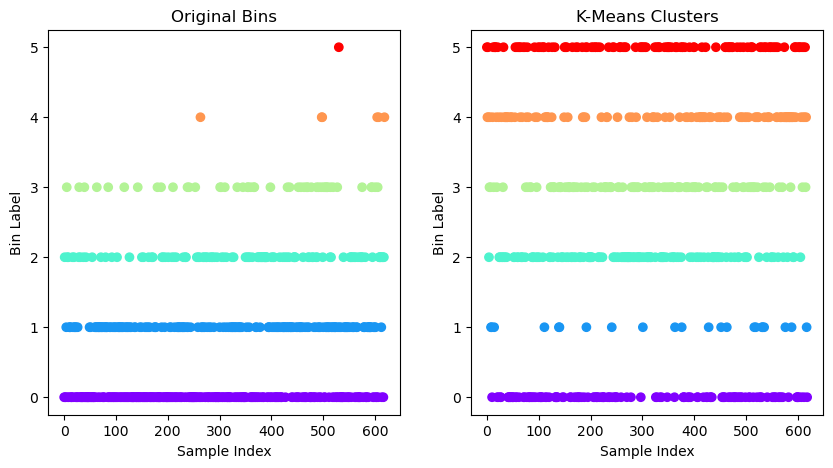
\includegraphics[width=0.7\linewidth]{files/c304de0d0bbb557996f173a0989550f1.png}

\subparagraph{Compute K-Means SSE}

\begin{verbatim}
# Compute SSE
SSE_kmeans = np.float64(kmeans.inertia_)
SSE_kmeans
\end{verbatim}

\begin{verbatim}
np.float64(1840.9904638055532)
\end{verbatim}

\subparagraph{DBSCAN Clustering}

\begin{verbatim}
# Set the number of clusters for K -means
k = int(number_of_bins)
y_bins = np.array(cleaned_meal_bin_indices)

# Initialize and fit KMeans
kmeans = KMeans(n_clusters=k, random_state=123)
y_kmeans = kmeans.fit_predict(scaled_meal_glucose_features_matrix)

# Get cluster labels and centroids
kmeans_cluster_labels = kmeans.labels_
centroids = kmeans.cluster_centers_

pca = PCA(n_components=2)
X_pca = pca.fit_transform(scaled_meal_glucose_features_matrix)

# Plotting the clusters found by k -means
plt.figure(figsize=(10, 5))

# Get the viridis color map and extract six colors from it
viridis = get_cmap('viridis', k)
colors = [viridis(i) for i in range(k)]

# Subplot 1: Scatter plot by k -means clusters
plt.subplot(1, 2, 1)
for i in range(k):
    cluster_points = X_pca[y_kmeans == i]
    plt.scatter(cluster_points[:, 0], cluster_points[:, 1], 
                color=colors[i], label=f'Cluster {i + 1}', alpha=0.6, marker='o')

# Plotting the centroids after PCA transformation
centroids_pca = pca.transform(centroids)
plt.scatter(centroids_pca[:, 0], centroids_pca[:, 1], 
            color='red', edgecolor='black', marker='X', s=100, label='Centroids')

plt.title("K -Means Clusters")
plt.xlabel('PCA Component 1')
plt.ylabel('PCA Component 2')
plt.legend()

# Get axis limits to keep the same scale for the second plot
x_lim = plt.xlim()
y_lim = plt.ylim()

# Subplot 2: Scatter plot by DBSCAN clusters
plt.subplot(1, 2, 2)

eps = 280  # Maximum distance between two points to be considered neighbors
min_samples = 15  # Minimum number of points in a neighborhood to form a dense region

dbscan = DBSCAN(eps=eps, min_samples=min_samples)
y_dbscan = dbscan.fit_predict(meal_glucose_features_matrix)

# Create a color palette for the clusters found by DBSCAN, including noise ( -1) as black
unique_labels = set(y_dbscan)
dbscan_colors = [plt.cm.viridis(float(i) / (max(unique_labels) if max(unique_labels) > 0 else 1))
                 for i in unique_labels]

# Color each point by DBSCAN cluster, use black for noise points
for label in unique_labels:
    if label == -1:
        # Noise points are labeled as -1
        plt.scatter(X_pca[y_dbscan == label, 0], X_pca[y_dbscan == label, 1], 
                    color='black', s=10, label='Noise', alpha=0.6, marker='x')
    else:
        plt.scatter(X_pca[y_dbscan == label, 0], X_pca[y_dbscan == label, 1], 
                    color=dbscan_colors[label], label=f'Cluster {label + 1}', alpha=0.6, marker='o')

plt.title("DBSCAN Clusters")
plt.xlabel('PCA Component 1')
plt.ylabel('PCA Component 2')
plt.xlim(x_lim)  # Apply same x -axis limits as K -means plot
plt.ylim(y_lim)  # Apply same y -axis limits as K -means plot
plt.legend()

plt.show()
\end{verbatim}

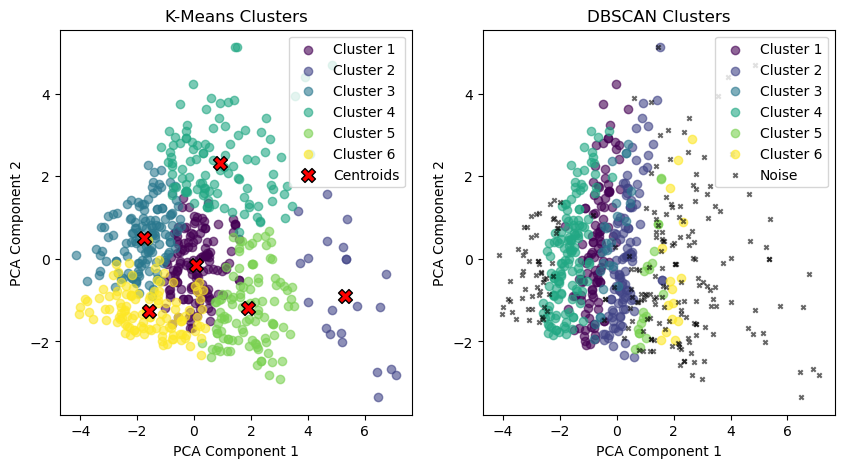
\includegraphics[width=0.7\linewidth]{files/ed96168d639b68c6f4d24814eeecdb9d.png}

\begin{verbatim}
y_bins = np.array(cleaned_meal_bin_indices)

# DBSCAN Parameters
eps = 280  # Maximum distance between two points to be considered neighbors
min_samples = 15  # Minimum number of points in a neighborhood to form a dense region

# Fit DBSCAN
dbscan = DBSCAN(eps=eps, min_samples=min_samples)
y_dbscan = dbscan.fit_predict(meal_glucose_features_matrix)

# Adjust labels to start from 0 (handle noise points separately)
# Noise points are marked as -1, so we'll make their label `max_label + 1`
adjusted_y_dbscan = y_dbscan.copy()
max_label = y_dbscan.max()

# Replace all noise labels ( -1) with a new label which is `max_label + 1`
adjusted_y_dbscan[adjusted_y_dbscan == -1] = max_label + 1

# Plotting the clusters found by DBSCAN and original bins
plt.figure(figsize=(10, 5))

# Subplot 1: Scatter plot by original bins
plt.subplot(1, 2, 1)
plt.scatter(
    np.arange(0, y_bins.shape[0]),
    y_bins,
    c=y_bins,
    cmap='rainbow',
    marker='o')
plt.title("Original Bins")
plt.xlabel("Sample Index")
plt.ylabel("Bin Label")

# Subplot 2: Scatter plot by DBSCAN clusters
plt.subplot(1, 2, 2)
plt.scatter(
    np.arange(0, adjusted_y_dbscan.shape[0]),
    adjusted_y_dbscan,
    c=adjusted_y_dbscan,
    cmap='rainbow',
    marker='o')
plt.title("DBSCAN Clusters")
plt.xlabel("Sample Index")
plt.ylabel("Cluster Label")

plt.tight_layout()
plt.show()
\end{verbatim}

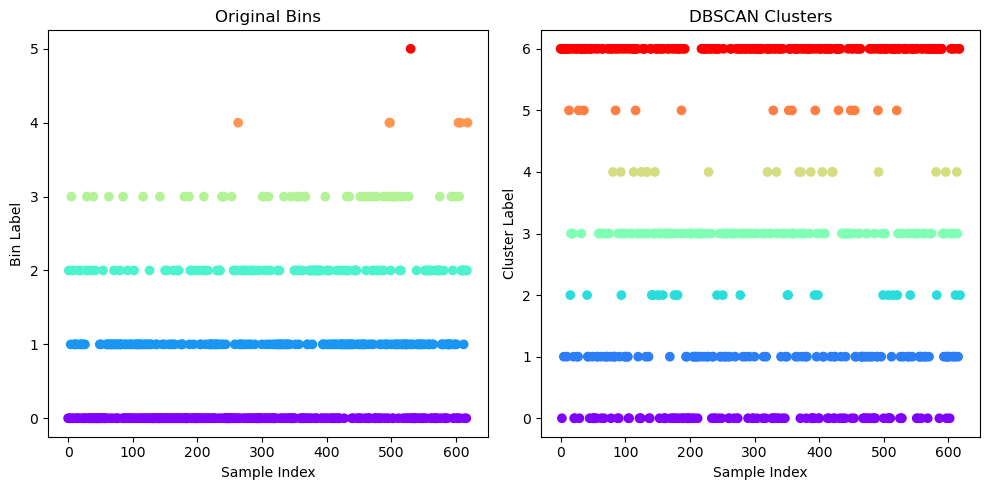
\includegraphics[width=0.7\linewidth]{files/6367ecbfbe24a5c604ce31af3284c456.png}

\subparagraph{Compute DBSCAN SSE}

\begin{verbatim}
# Get unique clusters excluding noise ( -1)
unique_clusters = set(y_dbscan) - { -1}

# Initialize SSE
SSE_dbscan = 0

# Loop over each cluster to compute SSE
for cluster in unique_clusters:
    # Get points in the current cluster
    cluster_points = meal_glucose_features_matrix[y_dbscan == cluster]
    
    # Compute the pseudo -centroid (mean of points in the cluster)
    pseudo_centroid = np.mean(cluster_points, axis=0)
    
    # Compute SSE for this cluster
    sse_cluster = np.sum((cluster_points - pseudo_centroid) ** 2)
    
    # Add the cluster's SSE to the total SSE
    SSE_dbscan += sse_cluster

print(f"Approximate SSE for DBSCAN (excluding noise): {SSE_dbscan}")
\end{verbatim}

\begin{verbatim}
Approximate SSE for DBSCAN (excluding noise): 365871520.5756363
\end{verbatim}

\subparagraph{Compute Entropy and Purity}

\subparagraph{K Means Cluster Bin Matrix}

\begin{verbatim}
df_kmeans_cluster = \
    pd.DataFrame(
        {'Cluster': kmeans_cluster_labels,
         'Bin': np.array(cleaned_meal_bin_indices)}
    )
df_kmeans_cluster
\end{verbatim}

\bigskip\noindent
\begin{tabular}{p{\dimexpr 0.333\linewidth-2\tabcolsep}p{\dimexpr 0.333\linewidth-2\tabcolsep}p{\dimexpr 0.333\linewidth-2\tabcolsep}}
\toprule
 & Cluster & Bin \\
\hline
0 & 5 & 0 \\
\hline
1 & 4 & 2 \\
\hline
2 & 5 & 0 \\
\hline
3 & 4 & 0 \\
\hline
4 & 2 & 1 \\
\hline
... & ... & ... \\
\hline
614 & 5 & 2 \\
\hline
615 & 3 & 2 \\
\hline
616 & 4 & 0 \\
\hline
617 & 1 & 2 \\
\hline
618 & 0 & 4 \\
\hline
\bottomrule
\end{tabular}

\bigskip

619 rows $\times$ 2 columns

\begin{verbatim}
df_kmeans_cluster_bin_matrix = \
    pd.crosstab(
        df_kmeans_cluster['Cluster'], 
        df_kmeans_cluster['Bin'])
df_kmeans_cluster_bin_matrix
\end{verbatim}

\bigskip\noindent
\begin{tabular}{p{\dimexpr 0.143\linewidth-2\tabcolsep}p{\dimexpr 0.143\linewidth-2\tabcolsep}p{\dimexpr 0.143\linewidth-2\tabcolsep}p{\dimexpr 0.143\linewidth-2\tabcolsep}p{\dimexpr 0.143\linewidth-2\tabcolsep}p{\dimexpr 0.143\linewidth-2\tabcolsep}p{\dimexpr 0.143\linewidth-2\tabcolsep}}
\toprule
Bin & 0 & 1 & 2 & 3 & 4 & 5 \\
\hline
Cluster &  &  &  &  &  &  \\
\hline
0 & 58 & 46 & 18 & 8 & 2 & 1 \\
\hline
1 & 7 & 5 & 5 & 5 & 0 & 0 \\
\hline
2 & 72 & 36 & 17 & 9 & 1 & 0 \\
\hline
3 & 41 & 30 & 24 & 11 & 0 & 0 \\
\hline
4 & 40 & 39 & 19 & 7 & 1 & 0 \\
\hline
5 & 56 & 27 & 25 & 7 & 2 & 0 \\
\hline
\bottomrule
\end{tabular}

\bigskip

\subparagraph{DBSCAN Cluster Bin Matrix}

\begin{verbatim}
#y_dbscan
\end{verbatim}

\begin{verbatim}
df_dbscan_cluster = \
    pd.DataFrame(
        {'Cluster': y_dbscan,
         'Bin': np.array(cleaned_meal_bin_indices)}
    )

df_dbscan_cluster = \
    df_dbscan_cluster[df_dbscan_cluster['Cluster'] != -1]
df_dbscan_cluster
\end{verbatim}

\bigskip\noindent
\begin{tabular}{p{\dimexpr 0.333\linewidth-2\tabcolsep}p{\dimexpr 0.333\linewidth-2\tabcolsep}p{\dimexpr 0.333\linewidth-2\tabcolsep}}
\toprule
 & Cluster & Bin \\
\hline
2 & 0 & 0 \\
\hline
5 & 1 & 3 \\
\hline
10 & 1 & 1 \\
\hline
13 & 5 & 0 \\
\hline
15 & 2 & 0 \\
\hline
... & ... & ... \\
\hline
612 & 1 & 1 \\
\hline
613 & 4 & 0 \\
\hline
614 & 3 & 2 \\
\hline
615 & 1 & 2 \\
\hline
618 & 2 & 4 \\
\hline
\bottomrule
\end{tabular}

\bigskip

403 rows $\times$ 2 columns

\begin{verbatim}
df_dbscan_cluster_bin_matrix = \
    pd.crosstab(
        df_dbscan_cluster['Cluster'], 
        df_dbscan_cluster['Bin'])
df_dbscan_cluster_bin_matrix
\end{verbatim}

\bigskip\noindent
\begin{tabular}{p{\dimexpr 0.143\linewidth-2\tabcolsep}p{\dimexpr 0.143\linewidth-2\tabcolsep}p{\dimexpr 0.143\linewidth-2\tabcolsep}p{\dimexpr 0.143\linewidth-2\tabcolsep}p{\dimexpr 0.143\linewidth-2\tabcolsep}p{\dimexpr 0.143\linewidth-2\tabcolsep}p{\dimexpr 0.143\linewidth-2\tabcolsep}}
\toprule
Bin & 0 & 1 & 2 & 3 & 4 & 5 \\
\hline
Cluster &  &  &  &  &  &  \\
\hline
0 & 41 & 37 & 19 & 9 & 0 & 0 \\
\hline
1 & 43 & 35 & 19 & 7 & 1 & 1 \\
\hline
2 & 16 & 2 & 2 & 4 & 1 & 0 \\
\hline
3 & 65 & 35 & 24 & 6 & 1 & 0 \\
\hline
4 & 10 & 6 & 3 & 1 & 0 & 0 \\
\hline
5 & 3 & 4 & 4 & 4 & 0 & 0 \\
\hline
\bottomrule
\end{tabular}

\bigskip

\subparagraph{Define Entropy Function}

\begin{verbatim}
def entropy(entries):
    entries = entries[entries > 0]
    return -np.sum(entries * np.log2(entries))
\end{verbatim}

\subparagraph{Calculate K Means Row Entropy Values}

\begin{verbatim}
k_means_entropy_values = \
    df_kmeans_cluster_bin_matrix.apply(lambda row: entropy(row / row.sum()), axis=1)
k_means_entropy_values
\end{verbatim}

\begin{verbatim}
Cluster
0    1.830430
1    1.983050
2    1.681496
3    1.869815
4    1.828204
5    1.816162
dtype: float64
\end{verbatim}

\subparagraph{Calculate DBSCAN Row Entropy Values}

\begin{verbatim}
dbscan_entropy_values = \
    df_dbscan_cluster_bin_matrix.apply(lambda row: entropy(row / row.sum()), axis=1)
dbscan_entropy_values
\end{verbatim}

\begin{verbatim}
Cluster
0    1.806700
1    1.886256
2    1.603856
3    1.716418
4    1.647731
5    1.989898
dtype: float64
\end{verbatim}

\subparagraph{Calculate Total Entropy}

\subparagraph{Calculate K Means Cluster Sizes}

\begin{verbatim}
k_means_cluster_sizes = df_kmeans_cluster_bin_matrix.sum(axis=1)
k_means_cluster_sizes
\end{verbatim}

\begin{verbatim}
Cluster
0    133
1     22
2    135
3    106
4    106
5    117
dtype: int64
\end{verbatim}

\subparagraph{Calculate DBSCAN Cluster Sizes}

\begin{verbatim}
dbscan_cluster_sizes = df_dbscan_cluster_bin_matrix.sum(axis=1)
dbscan_cluster_sizes
\end{verbatim}

\begin{verbatim}
Cluster
0    106
1    106
2     25
3    131
4     20
5     15
dtype: int64
\end{verbatim}

\subparagraph{Total Data Points}

\begin{verbatim}
total_data_points = len(meal_glucose_features_matrix)
total_data_points
\end{verbatim}

\begin{verbatim}
619
\end{verbatim}

\subparagraph{K-Means Total Entropy}

\begin{verbatim}
k_means_total_entropy = \
    np.sum(k_means_cluster_sizes * k_means_entropy_values) / total_data_points
k_means_total_entropy
\end{verbatim}

\begin{verbatim}
np.float64(1.807039149934111)
\end{verbatim}

\subparagraph{DBSCAN Total Entropy}

\begin{verbatim}
dbscan_total_entropy = \
    np.sum(dbscan_cluster_sizes * dbscan_entropy_values) / total_data_points
dbscan_total_entropy
\end{verbatim}

\begin{verbatim}
np.float64(1.161879812576486)
\end{verbatim}

\subparagraph{Calculate Total Purity}

\subparagraph{Calculate K Means Purity Values}

\begin{verbatim}
k_means_purity_values = \
    df_kmeans_cluster_bin_matrix.apply(lambda row: row.max() / row.sum(), axis=1)
k_means_purity_values
\end{verbatim}

\begin{verbatim}
Cluster
0    0.436090
1    0.318182
2    0.533333
3    0.386792
4    0.377358
5    0.478632
dtype: float64
\end{verbatim}

\subparagraph{Calculate DBSCAN Purity Values}

\begin{verbatim}
dbscan_purity_values = \
    df_dbscan_cluster_bin_matrix.apply(lambda row: row.max() / row.sum(), axis=1)
dbscan_purity_values
\end{verbatim}

\begin{verbatim}
Cluster
0    0.386792
1    0.405660
2    0.640000
3    0.496183
4    0.500000
5    0.266667
dtype: float64
\end{verbatim}

\subparagraph{K-Means Total Purity}

\begin{verbatim}
k_means_total_purity = \
    np.sum(k_means_cluster_sizes * k_means_purity_values) / total_data_points
k_means_total_purity
\end{verbatim}

\begin{verbatim}
np.float64(0.44264943457189015)
\end{verbatim}

\subparagraph{DBSCAN Total Purity}

\begin{verbatim}
dbscan_total_purity = \
    np.sum(dbscan_cluster_sizes * dbscan_purity_values) / total_data_points
dbscan_total_purity
\end{verbatim}

\begin{verbatim}
np.float64(0.28917609046849757)
\end{verbatim}

\subparagraph{Create Results File}

\begin{verbatim}
results = [
    SSE_kmeans,
    SSE_dbscan,
    k_means_total_entropy,
    dbscan_total_entropy,
    k_means_total_purity,
    dbscan_total_purity
]
results
\end{verbatim}

\begin{verbatim}
[np.float64(1840.9904638055532),
 np.float64(365871520.5756363),
 np.float64(1.807039149934111),
 np.float64(1.161879812576486),
 np.float64(0.44264943457189015),
 np.float64(0.28917609046849757)]
\end{verbatim}

\begin{verbatim}
results_matrix_1x6 = np.array(results).reshape(1, 6)
results_matrix_1x6
\end{verbatim}

\begin{verbatim}
array([[1.84099046e+03, 3.65871521e+08, 1.80703915e+00, 1.16187981e+00,
        4.42649435e -01, 2.89176090e -01]])
\end{verbatim}

\begin{verbatim}
np.savetxt('Result.csv', results_matrix_1x6, delimiter=',', fmt='%10.5f')
\end{verbatim}